\documentclass[a4wide,10pt,twocolumn]{article}
\usepackage{a4wide,url,longtable,lscape,verbatim,amsmath,amssymb,graphicx,multirow,fancyhdr,lastpage,algorithm2e}
\usepackage[font=small,format=plain,labelfont=bf,up,textfont=it,up]{caption}


% --- Informal Requirements Commands ---
\newcounter{req_count}
\setcounter{req_count}{1}


\newcommand{\course}{Additional Component Computer Graphics (2IV05)}
\newcommand{\student}{\footnotesize Page \thepage~of \pageref{LastPage}}
\newcommand{\subject}{Final report}

\fancypagestyle{plain}{%
\fancyhf{} %
\fancyfoot[C]{\student} %
\fancyhead[LE, RO]{\subject} %
\fancyhead[LO, RE]{\course} %
}

\pagestyle{fancy}{%
\fancyhf{} %
\fancyfoot[C]{\student} %
\fancyhead[LE, RO]{\subject} %
\fancyhead[LO, RE]{\course} %

% Used commands
\newcommand{\Bound}{\mbox{Bound}}

% Nice algorithm styles
\linesnumbered
\dontprintsemicolon
\SetLine

% No paragraph indent, it's ugly
\setlength\parindent{0em}
\setlength\parskip{0.8em}

% Make sure no text goes beyond the page
\setlength{\textheight}{60em}

%opening
\title{2IV05 - Additional Component Computer Graphics \\ Final Report}
\author{Bart van Arnhem (0557184) \\ Maarten Manders (0573419)}

\begin{document}
\maketitle
\thispagestyle{empty}

\onecolumn
\tableofcontents
\setcounter{page}{1}
\twocolumn
\section{Introduction}
This report describes the work that we have done for the Additional Component Computer Graphics course (2IV05). We have written a program called \emph{CSGBuilder} which allows a user to create complex three-dimensional objects using only a small number of simple primitives, which are basically simple objects.

We have used a technique, called Constructive Solid Geometry, or CSG in short, to create our models. This technique uses mathematical functions to represent primitives and boolean operators to construct extended objects using these primitives.

For the rendering of our objects we used the adaptive marching cubes algorithm. This algorithm divides the space around the CSG objects in a number of cubes and constructs a mesh that approaches the form of the object. We have used the adaptive form of this algorithm, because this increases the precision of the rendered objects.

The rest of this document will describe the techniques that were mentioned above in more detail. Also the way we used the techniques will be explained. Besides this, the architecture and user interface of our program are explained.

We have used the Java\textcopyright\ programming language in combination with Swing and the Java OpenGL\texttrademark\ API (JOGL) to write our program. To increase the responsiveness of our program we used the JOGL AWT GLCanvas instead of the Swing GLJPanel, because the drawing on the AWT component is faster.

\section{Requirements}
\begin{figure*}[t!]
\centering
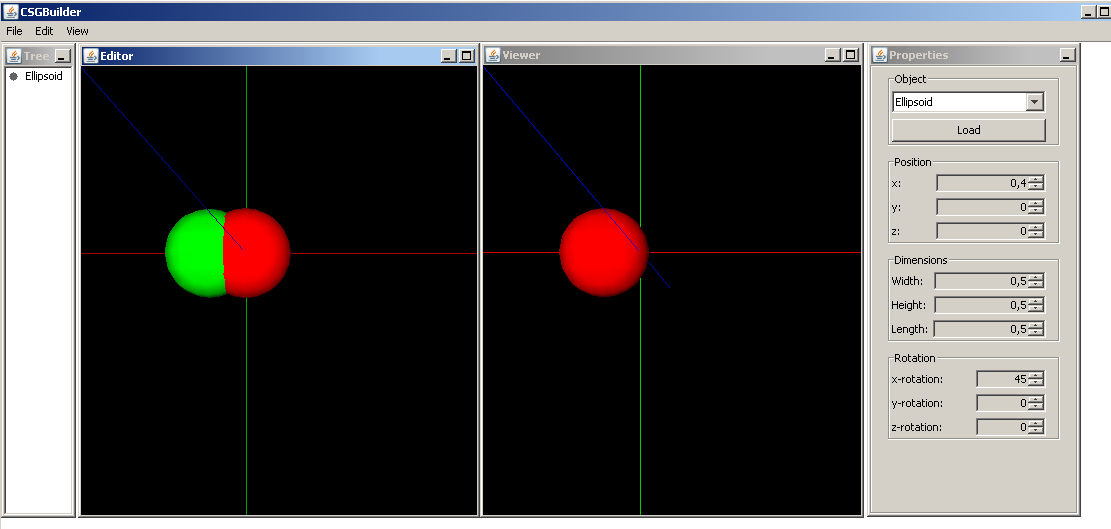
\includegraphics[width = 0.9\textwidth]{images/gui}
\caption{Actual GUI of current application}
\label{figure:gui}
\end{figure*}
This chapter is divided in two sections, in which different aspects of our system are specified as originally provided in our proposal. The ``Functionality'' section describes the functionality of \emph{CSGBuilder}. The ``Interaction and presentation'' section describes the ways how the users of our software can interact with \emph{CSGBuilder}.

\subsection{Functionality}
This section describes the functionality of the program. There are two kinds of functionality that will be added. ``Core functionality'' is that part of the software that must be implemented in order to make it work properly. ''Extra functionality'' is that part of the software that makes it more appealing. If time permits, all the functionality will be implemented, otherwise parts of the extra functionality will be dropped.

The core functionality consists of: \\
\vspace{-10pt}
\begin{enumerate}
    \setlength{\itemsep}{-0.3em}
	\item Object editing window
	\item Object selector window
	\item Object loading
	\item Object saving
	\item Shape Union
	\item Shape intersection
	\item Shape difference
	\item Zooming
	\item Rotation
\end{enumerate}
\bigskip
The extra functionality consists of: \\
\vspace{-10pt}
\begin{enumerate}
    \setlength{\itemsep}{-0.3em}
	\item Texturing
	\item Adding temporary shapes
	\item Preview
	\item Lighting
\end{enumerate}

\subsubsection{Possible extra functionality}
Possibility to specify a ``weight'', meaning only a certain amount of material is added or removed from the geometric object.

\subsection{Interaction and presentation}

%\begin{figure}[h]
%\centering
%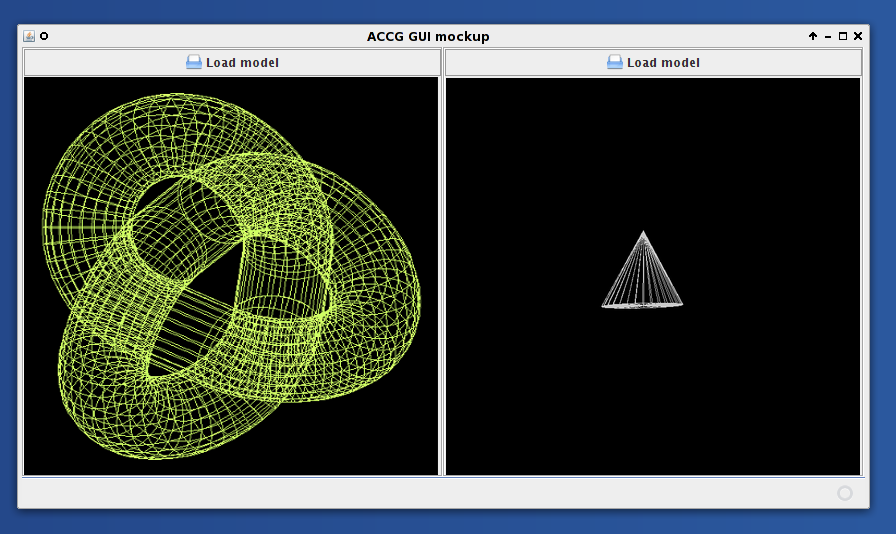
\includegraphics[width = 0.48\textwidth]{../resources/gui_mockup/1}
%\caption{\emph{Mockup of the graphical user interface}} \label{gui_mockup}
%\end{figure}


Figure \ref{figure:gui} displays a the graphical user interface of the application. Two main parts of the are the two windows displaying rendered objects. Displayed are the constructed object on the left and the building block object on the right. As described more complex object can be created by adding or removing the building block object from the constructed object.

Changing the view port on both windows can be done intuitively by dragging the mouse to rotate, or using the mouse wheel to zoom in or out of the object. By holding down the CTRL key while dragging the mouse the object can be translated. Resetting the view port to it's original state can be done by clicking somewhere inside the view port using the right mouse button.

When holding down the ALT or SHIFT key, the building block object appears in green in the same window as the constructed object (as displayed in Figure \ref{figure:gui}). The green object indicates where the building object is going to be added to, or removed from the constructed object. Actual adding of the object can be done by holding down the SHIFT key and clicking the left mouse button, holding down the ALT key and clicking will remove the object from the constructed object.

On the right there is a panel which allows the users to adjust certain parameters of the building block object like position ($x, y, z$), dimension (width, height, length) and the rotation (x, y, z axis). Adjusting this parameters will cause the building block object to be re-rendered and will also influence the position at which the object is removed/added from the constructed object. Also the panel has a \textit{Load} button which allows the user to load any previously constructed object and use it as a building block. Constructed objects can be saved by selecting \textit{Save} from the \textit{File} menu.

\section{Representing Objects}
\label{chapt:repobj}


    \begin{table*}[t!]
        \begin{tabular}{|p{.1\linewidth}|p{.41\linewidth}|p{.40\linewidth}|}
            \hline
            \textbf{Primitive} & \textbf{Description} & \textbf{Formula}\\
            \hline
            \hline
             \vspace{0.1em}
             Ellipsoid &
             \vspace{0.1em}
             Spheres or cigar formed shapes &
             \vspace{0.1em}
             $f(x,y,z)=(\frac{p_x + x}{r_x})^2+(\frac{p_x + x}{r_x})^2+(\frac{p_x + x}{r_x})^2 - 1$\\[1.2em]
            \hline
             \vspace{0.1em}
             Cuboid &
             \vspace{0.1em}
             Rectangles or bars with rounded corners &
             \vspace{0.1em}
             $f(x,y,z)=(\frac{p_x + x}{r_x})^4+(\frac{p_x + x}{r_x})^4+(\frac{p_x + x}{r_x})^4 - 1$\\[1.2em]
            \hline
        \end{tabular}
        \caption{The primitives of CSGBuilder}
        \label{table:primitives}
    \end{table*}


\subsection{CSG Tree}
    To represent the objects that are modeled with our program, the Constructive Solid Geometry (CSG) technique is used. This technique uses a number of simple objects, called primitives, that are combined in to more complex objects by using boolean operators. To represent the CSG objects the CSG trees that are described in \cite{Wiegand96} are used. Figure~\ref{figure:csg_tree} shows an example of a simple CSG tree.

    \begin{figure}[h]
        \begin{center}
            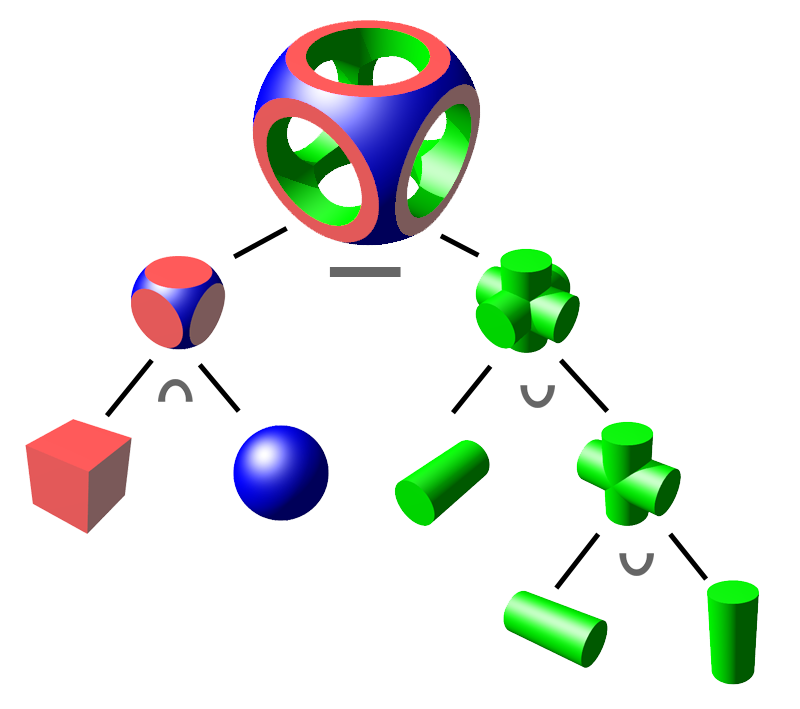
\includegraphics[scale=.2]{./images/csgtree.png}
        \end{center}
        \caption{An example of a CSG tree (source: wikipedia\cite{img:wiki_csg_tree})}
        \label{figure:csg_tree}
    \end{figure}

    In a CSG tree the boolean operators are the nodes in a binary tree and the primitives are the leaves of the tree. The primitives are represented by mathematical functions in $\mathbb{R}^3$. The operators combine the primitives in a object by using boolean functions on the results of the primitive functions. How this is done will be explained in the next sections.

\subsubsection{Primitives}
    A primitive in a CSG tree is a function $A:\mathbb{R}^3 \rightarrow \mathbb{R}$. The form of an object is constructed by drawing the points $(x,y,z)$ for which $A(x,y,z)=0$. Our program has a small number of primitives, these are described in Table~\ref{table:primitives}. In this table $p_x$, $p_y$ and $p_z$ denote the coordinates of the position of the center of the primitive and $r_x$, $r_y$ and $r_z$ denote the size of the primitive in respectively the $x$, $y$ and $z$ direction. $e_x$, $e_y$ and $e_z$ denote exponents which define the shape of an object.

    These primitives can be rotated with arbitrary angels around all axes by multiplying a rotation matrix $R$, which is shown in Figure~\ref{figure:rotation_matrix}, with the vector $\overrightarrow{v}=(x,y,z)^T$, so the rotated point $\overrightarrow{w}=R\overrightarrow{v}$. Applying a primitive function $A$ on $\overrightarrow{w}^T$ causes the primitive to be rotated with angles $\alpha_x$, $\alpha_y$ and $\alpha_z$ around respectively the $x$, $y$ and $z$ axes.

    \begin{figure*}[!t]
    {\fontsize{8}{10}\selectfont
        \[
            \left(
                \begin{array}{lll}
                    \cos(\alpha_y)\cos(\alpha_z) &
                    \cos(\alpha_y)\sin(\alpha_z) &
                    -\sin(\alpha_y) \\

                    \sin(\alpha_x)\sin(\alpha_y)\cos(\alpha_z) - \cos(\alpha_x)\sin(\alpha_z) &
                    \sin(\alpha_x)\sin(\alpha_y)\sin(\alpha_z) + \cos(\alpha_x)\cos(\alpha_z) &
                    \sin(\alpha_x)\cos(\alpha_y) \\

                    \cos(\alpha_x)\sin(\alpha_y)\cos(\alpha_z) + \sin(\alpha_x)\sin(\alpha_z) &
                    \cos(\alpha_x)\sin(\alpha_y)\sin(\alpha_z) - \sin(\alpha_x)\cos(\alpha_z) &
                    \cos(\alpha_x)\cos(\alpha_y) \\
                \end{array}
            \right)
        \]}
        \caption{The rotation matrix $R$}
        \label{figure:rotation_matrix}
    \end{figure*}

\subsubsection{Operators}
    There are three operations that can be used to construct a CSG tree. These are the union($\cup$), intersection($\cap$) and difference($-$) set operations. These set operations have to be mapped to the mathematical functions of which CSG trees are constructed, this can be done using the $\min$ and $\max$ functions, as can be seen in Figure~\ref{figure:operations}. In the figure $A, B:\mathbb{R}^3 \rightarrow \mathbb{R}$ are functions (possibly CSG trees) of which a CSG tree is constructed.

    \begin{figure}[h]
        {\fontsize{8.7}{10}\selectfont
        \textbf{Union:}\\
        $A \cup B: \forall[x,y,z \in \mathbb{R} :: \min(A(x, y, z), B(x, y, z))]$ \\

        \textbf{Intersection:}\\
        $A \cap B: \forall[x,y,z \in \mathbb{R} :: \max(A(x, y, z), B(x, y, z))]$ \\

        \textbf{Difference:}\\
        $A - B: \forall[x,y,z \in \mathbb{R} :: \max(A(x, y, z), -B(x, y, z))]$
        }
        \caption{The operations to construct CSG trees}
        \label{figure:operations}
    \end{figure}

    By combining the primitives with the operators, it is possible to create complex objects. When these objects consist of many primitives and operators the rendering of the object tends to be slow. It is possible increase the rendering speed by creating a normalize CSG tree. A way in which CSG trees can be normalized is described in the next section.

\subsubsection{Normalizing CSG trees}
    As described in \cite{Wiegand96}, it is possible to increase the rendering speed, by normalizing CSG trees to a \textit{sum of products} form. This means that that all intersection and difference operators have a left subtree which contains no union operators and a right subtree that consists of a primitive. To create a normalized CSG tree, the nine operations that are described in \cite{Wiegand96} are used. These operations are recalled in Figure~\ref{table:normalize}.

    \begin{table}[h]
        \begin{tabular}{llll}
            1. & $X - (Y \cup Z)$    & $\rightarrow$ & $(X - Y) - Z$\\
            2. & $X \cap (Y \cup Z)$ & $\rightarrow$ & $(X \cap Y) \cup (X \cap Z)$\\
            3. & $X - (Y \cap Z)$    & $\rightarrow$ & $(X - Y) \cup (X - Z)$\\
            4. & $X \cap (Y \cap Z)$ & $\rightarrow$ & $(X \cap Y) \cap Z$\\
            5. & $X - (Y - Z)$       & $\rightarrow$ & $(X - Y) \cup (X \cap Z)$\\
            6. & $X \cap (Y - Z)$    & $\rightarrow$ & $(X \cap Y) - Z$\\
            7. & $(X - Y) \cap Z$    & $\rightarrow$ & $(X \cap Z) - Y$\\
            8. & $(X \cup Y) - Z$    & $\rightarrow$ & $(X - Z) \cup (Y - Z)$\\
            9. & $(X \cup Y) \cap Z$ & $\rightarrow$ & $(X \cap Z) \cup (Y \cap Z)$\\
        \end{tabular}
        \caption{Operations to normalize a CSG tree}
        \label{table:normalize}
    \end{table}

    When the normalization is completed, the CSG tree might contain nodes which could be rendered even faster. The normalized CSG tree could be pruned according to the operations that are stated in Table~\ref{table:prune}. The pruning of the tree leads to less calculations, so the time that is needed to render the object is decreased.

    \begin{table}[h]
        \hspace{-0.8em}
        \begin{tabular}{p{0.01\textwidth} p{0.12\textwidth} p{0.31\textwidth} }
            1. & $A \cap B \rightarrow \emptyset$ & if $\Bound(A)$ does not intersect $\Bound(B)$\\
            2. & $A - B \rightarrow A$            & if $\Bound(A)$ does not intersect $\Bound(B)$\\
        \end{tabular}
        \caption{Operations to prune a normalized CSG tree}
        \label{table:prune}
    \end{table}

    In order to decide whether a node in the tree should be pruned, the cases in which the pruning takes place should be recognized. This can be done by constructing and calculating the bounding boxes of nodes in the CSG tree. The bounding box $\Bound$ of a primitive is simply the smallest cube in which the primitive can be placed. To determine the bounding box of operations in the CSG tree the equations in Table~\ref{table:bounding_box} can be used.

    \begin{table}[h]
        {\fontsize{8.7}{10}\selectfont
            1. $\Bound(A \cup B) = \Bound(\Bound(A) \cup \Bound(B))$\\
            2. $\Bound(A \cap B) = \Bound(\Bound(A) \cap \Bound(B))$\\
            3. $\Bound(A - B)    = \Bound(A)$\\
        }
        \caption{The computation of a bounding box of a CSG tree}
        \label{table:bounding_box}
    \end{table}

    Applying the normalization and pruning operations on the nodes of a tree leads to the normalization algorithm that is described in  Figure~\ref{figure:algorithm}. This algorithm is based on the normalization algorithm in \cite{Wiegand96}.

    \begin{figure}[ht]
            \textbf{Algorithm} $\textsc{Normalize}(T: CSGTree)$\\
            \noindent
            \begin{algorithm}[H]
                \If{$T$ is a primitive}{
                    \Return\;
                }
                \BlankLine
                \Repeat{($T\mbox{.op is a union}) \lor ((T\mbox{.right is a primitive}) \land (T\mbox{.left is not a union}))$}{
                    \Repeat{$\neg changed$}{
                        $changed \gets \textsc{False}$\;
                        \If{$T$ matches a rule from Figure~\ref{table:normalize}} {
                            Apply the first matching rule\;
                            $changed \gets \textsc{True}$\;
                        }
                    }
                    \textsc{Normalize}$(T\mbox{.left})$\;
                    \textsc{Prune}$(T)$\;
                }
                \BlankLine
                \textsc{Normalize}$(T\mbox{.right})$\;
            \end{algorithm}
        \caption{The algorithm that generates a normalized CSG tree}
        \label{figure:algorithm}
    \end{figure}

\section{Rendering Objects}

As described in previous chapter (chapter \ref{chapt:repobj}) our objects are internally stored as CSG tree's, essentially a combination of implicit volumes resulting in a more complex object.

We are rendering these objects using the marching cubes algorithm. Given an implicit volume, the marching cubes algorithm will return a mesh that approximates the volume. It does this by dividing the space into a number of cubes and then visit each cube individually which of the corners are inside or outside of the volume. This depends on the value of the implicit function at that point. Using this it can determine where triangles should be placed. This is described in more detail in the following sections.

\subsection{Adaptive Marching Cubes}

The standard marching cubes algorithm will divide the 3d space into a number of cubes all of the same dimension. This works for most objects, but as the features of the objects get sharper (for example sharp edges) we need smaller sized cubes (which means more) to get an acceptable level of detail on the rendered object. Of course the more cubes, the slower the algorithm will be.

Because still most of the object will be relatively flat compared to the sharp features it would be a better idea to only have finer grained cubes where needed, thus at places where the sharp features of the objects are. With this extension we get an adaptive form of the marching cubes algorithm.

\subsubsection{Octree}

An octree is essentially a tree data structure where every node has eight child nodes (if any). In our case a node is a cube and it children are the cube divided into eight equally sized smaller cubes (see figure \ref{figure:octree}).

    \begin{figure}[h]
        \begin{center}
            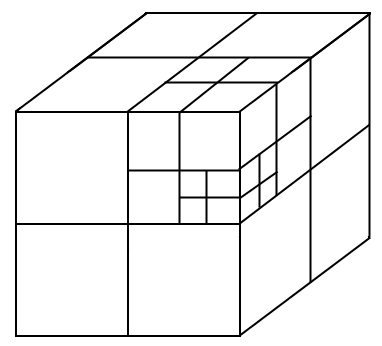
\includegraphics[scale=0.4]{./images/octree_block}
        \end{center}
        \caption{Bounding box subdivision example}
        \label{figure:octree}
    \end{figure}

This is exactly what we need to divide our 3d space into a number of cubes, and have finer grained cubes in area's where the object has sharp features.

\subsubsection{Construction of the octree}
\label{sect:genoctree}
Initially we start by taking the bounding box of the object that has to be triangulated and set it's bounding box as the root of the octree. The bounding box can be is already calculated for us by the CSG tree. To get the algorithm started the first two recursions are always done. One recursion means that a cube is divided into eight sub cubes. So the 3d space is always divided into at least $8 \cdot 8 = 64$ cubes.

The next step is to visit each leaf node, and check if the part of the volume that is inside the cube for this node has any sharp features, if so another recursion step is done. This sharpness check is done by triangulating the cube (by marching the cube once) and collecting the vertices. If all normals for these vertices point approximately in the same direction, it means the surface can be considered "flat" and we do not need to recurse.

    \begin{figure}[h]
        \begin{center}
            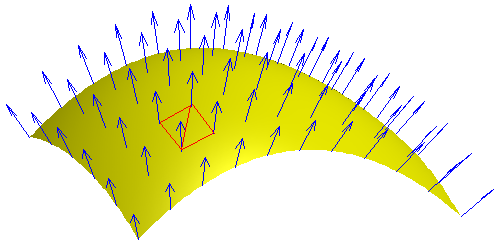
\includegraphics[scale=0.4]{./images/Surface_normal}
        \end{center}
        \caption{Example surface normals (source$^1$)}
        \label{figure:surface_normal}
    \end{figure}

To determine if the volume inside a cube has sharp features we use the following algorithm with input $N$ is the vertices collected from the triangles inside the cube:

    \begin{figure}[ht]
            \textbf{Algorithm} $\textsc{IsSharp}(N: Vertices)$\\
            \noindent
            \begin{algorithm}[H]
                \CommentSty{// N is a list of vertices}\;
                \For{every pair $v, w \in N$ where $v \neq w$}{
                    \If{$arccos(dot\_product(v, w)) > \delta$} {
                        \Return{\textbf{true}}\;
                    }
                }
                \BlankLine
                \Return{\textbf{true}}\;
            \end{algorithm}
        \caption{Algorithm to detect if the volume inside a cube has sharp features}
        \label{figure:algorithm}
    \end{figure}

Essentially this algorithm returns true if the angle between any two vertices is larger than $\delta$. Given the definition of the dot product (see Figure \ref{figure:dot_product}). We can calculate the angle between $v$ and $w$ using the inverse cosine in the following way:
\footnotetext[1]{http://en.wikipedia.org/wiki/Surface\_normal}

\begin{equation}
    \theta = arccos(\displaystyle\frac{v \bullet w}{|v||w|})
\end{equation}

Because the vertices are normalized $|v||w|$ will always be $1$, so we can simplify this to $\theta = arccos(v \bullet w)$.

    \begin{figure}[h!]
        \begin{center}
            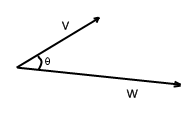
\includegraphics[scale=0.8]{./images/dotproduct}
        \end{center}
        \caption{Dot product $v \bullet w = |v||w|cos(\theta)$}
        \label{figure:dot_product}
    \end{figure}


\subsubsection{The algorithm}

The octree, generated as described in section \ref{sect:genoctree}, is used as the input for the algorithm. For every leaf node, the algorithm will march the cube assigned to that leaf node.

    \begin{figure}[h]
        \begin{center}
            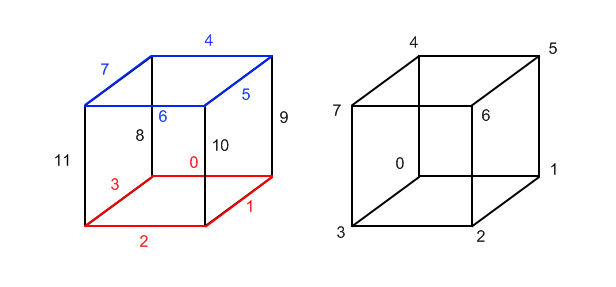
\includegraphics[scale=0.6]{./images/cube_config}
        \end{center}
        \caption{Cube A shows the edge configuration, cube B the vertex configuration}
        \label{figure:cube_config}
    \end{figure}

Each of the eight corner points of the cube can be either inside or outside of the implicit volume, this can be determined by the value returned by the CSG tree for these points. If the value is lower than the ISO value it means the point is inside the volume, else it's outside. So in total, because ever point can be either inside or outside of the volume, there are $2^8 = 256$ different cases.

The algorithm used two predefined lookup tables:

\begin{itemize}
    \item[] \textbf{Edge table} Contains a 12-bit number of every case, where the $i^{th}$ bit being $1$ means that the $i^{th}$ edge of the cube is cut by the implicit volume, so one endpoint of the edge is inside the volume and the other one is outside. If the bit is $0$ the edge is not cut.
    \item[] \textbf{Triangle table} Contains a list of edge indexes for every case. Every consecutive two edge indexes connect a side of a triangle from the first edge to the second edge.
\end{itemize}

The index to these lookup tables is calculated by setting the $i^{th}$ most significant bit to one if the $i^{th}$ corner vertex is inside the volume, else it's set to zero. Now using this index the algorithm can look at the \textbf{Edge table} and find all edges that are cut by the volume. For each edge that is indeed cut by the volume it will approximate the exact intersection point on the edge by using linear interpolation between the two endpoint of the edge:

\begin{eqnarray}
    p_e.x & = & p_i.x + r \cdot (p_o.x - p_i.x) \\
    p_e.y & = & p_i.y + r \cdot (p_o.y - p_i.y) \\
    p_e.z & = & p_i.z + r \cdot (p_o.z - p_i.z)
\end{eqnarray}

Where $p_e$, $p_i$ and $p_o$ are the approximated intersection point, the corner point inside the volume and the corner point outside of the volume respectively. $r$ is the interpolation ratio given by:

\begin{equation}
    r = (i - v_{p_i}) / (v_{p_o} - v_{p_i})
\end{equation}

Where $i$ is the ISO level (usually 0) and $v_{p_o}$ and $v_{p_i}$ are the values returned by the CSG tree for the two endpoints.

Next step in the algorithm is to walk through the list of triangle vertices defined in the \textbf{Triangle table}. These are already ordered to form a triangle so we can just take the approximated intersection point for this edge, which is calculated in previous step, and add this as a vertex.

\subsubsection{The crack problem}
\label{sect:crack_problem}

Cracks in the mesh can occur when neighboring cubes in the octree are not of the same resolution. When doing the interpolation step, or in non-flat areas the generated triangles in neighboring cubes will not exactly fit each other, causing visible cracks in the mesh. See figure \ref{fig:amccracks} for an example.

    \begin{figure}[h]
        \begin{center}
            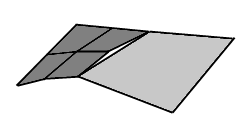
\includegraphics[scale=0.8]{./images/amccrack}
        \end{center}
        \caption{Example of a crack in the mesh caused by different resolution cubes}
        \label{figure:amccracks}
    \end{figure}

\section{Architecture}
\begin{figure*}[!t]
    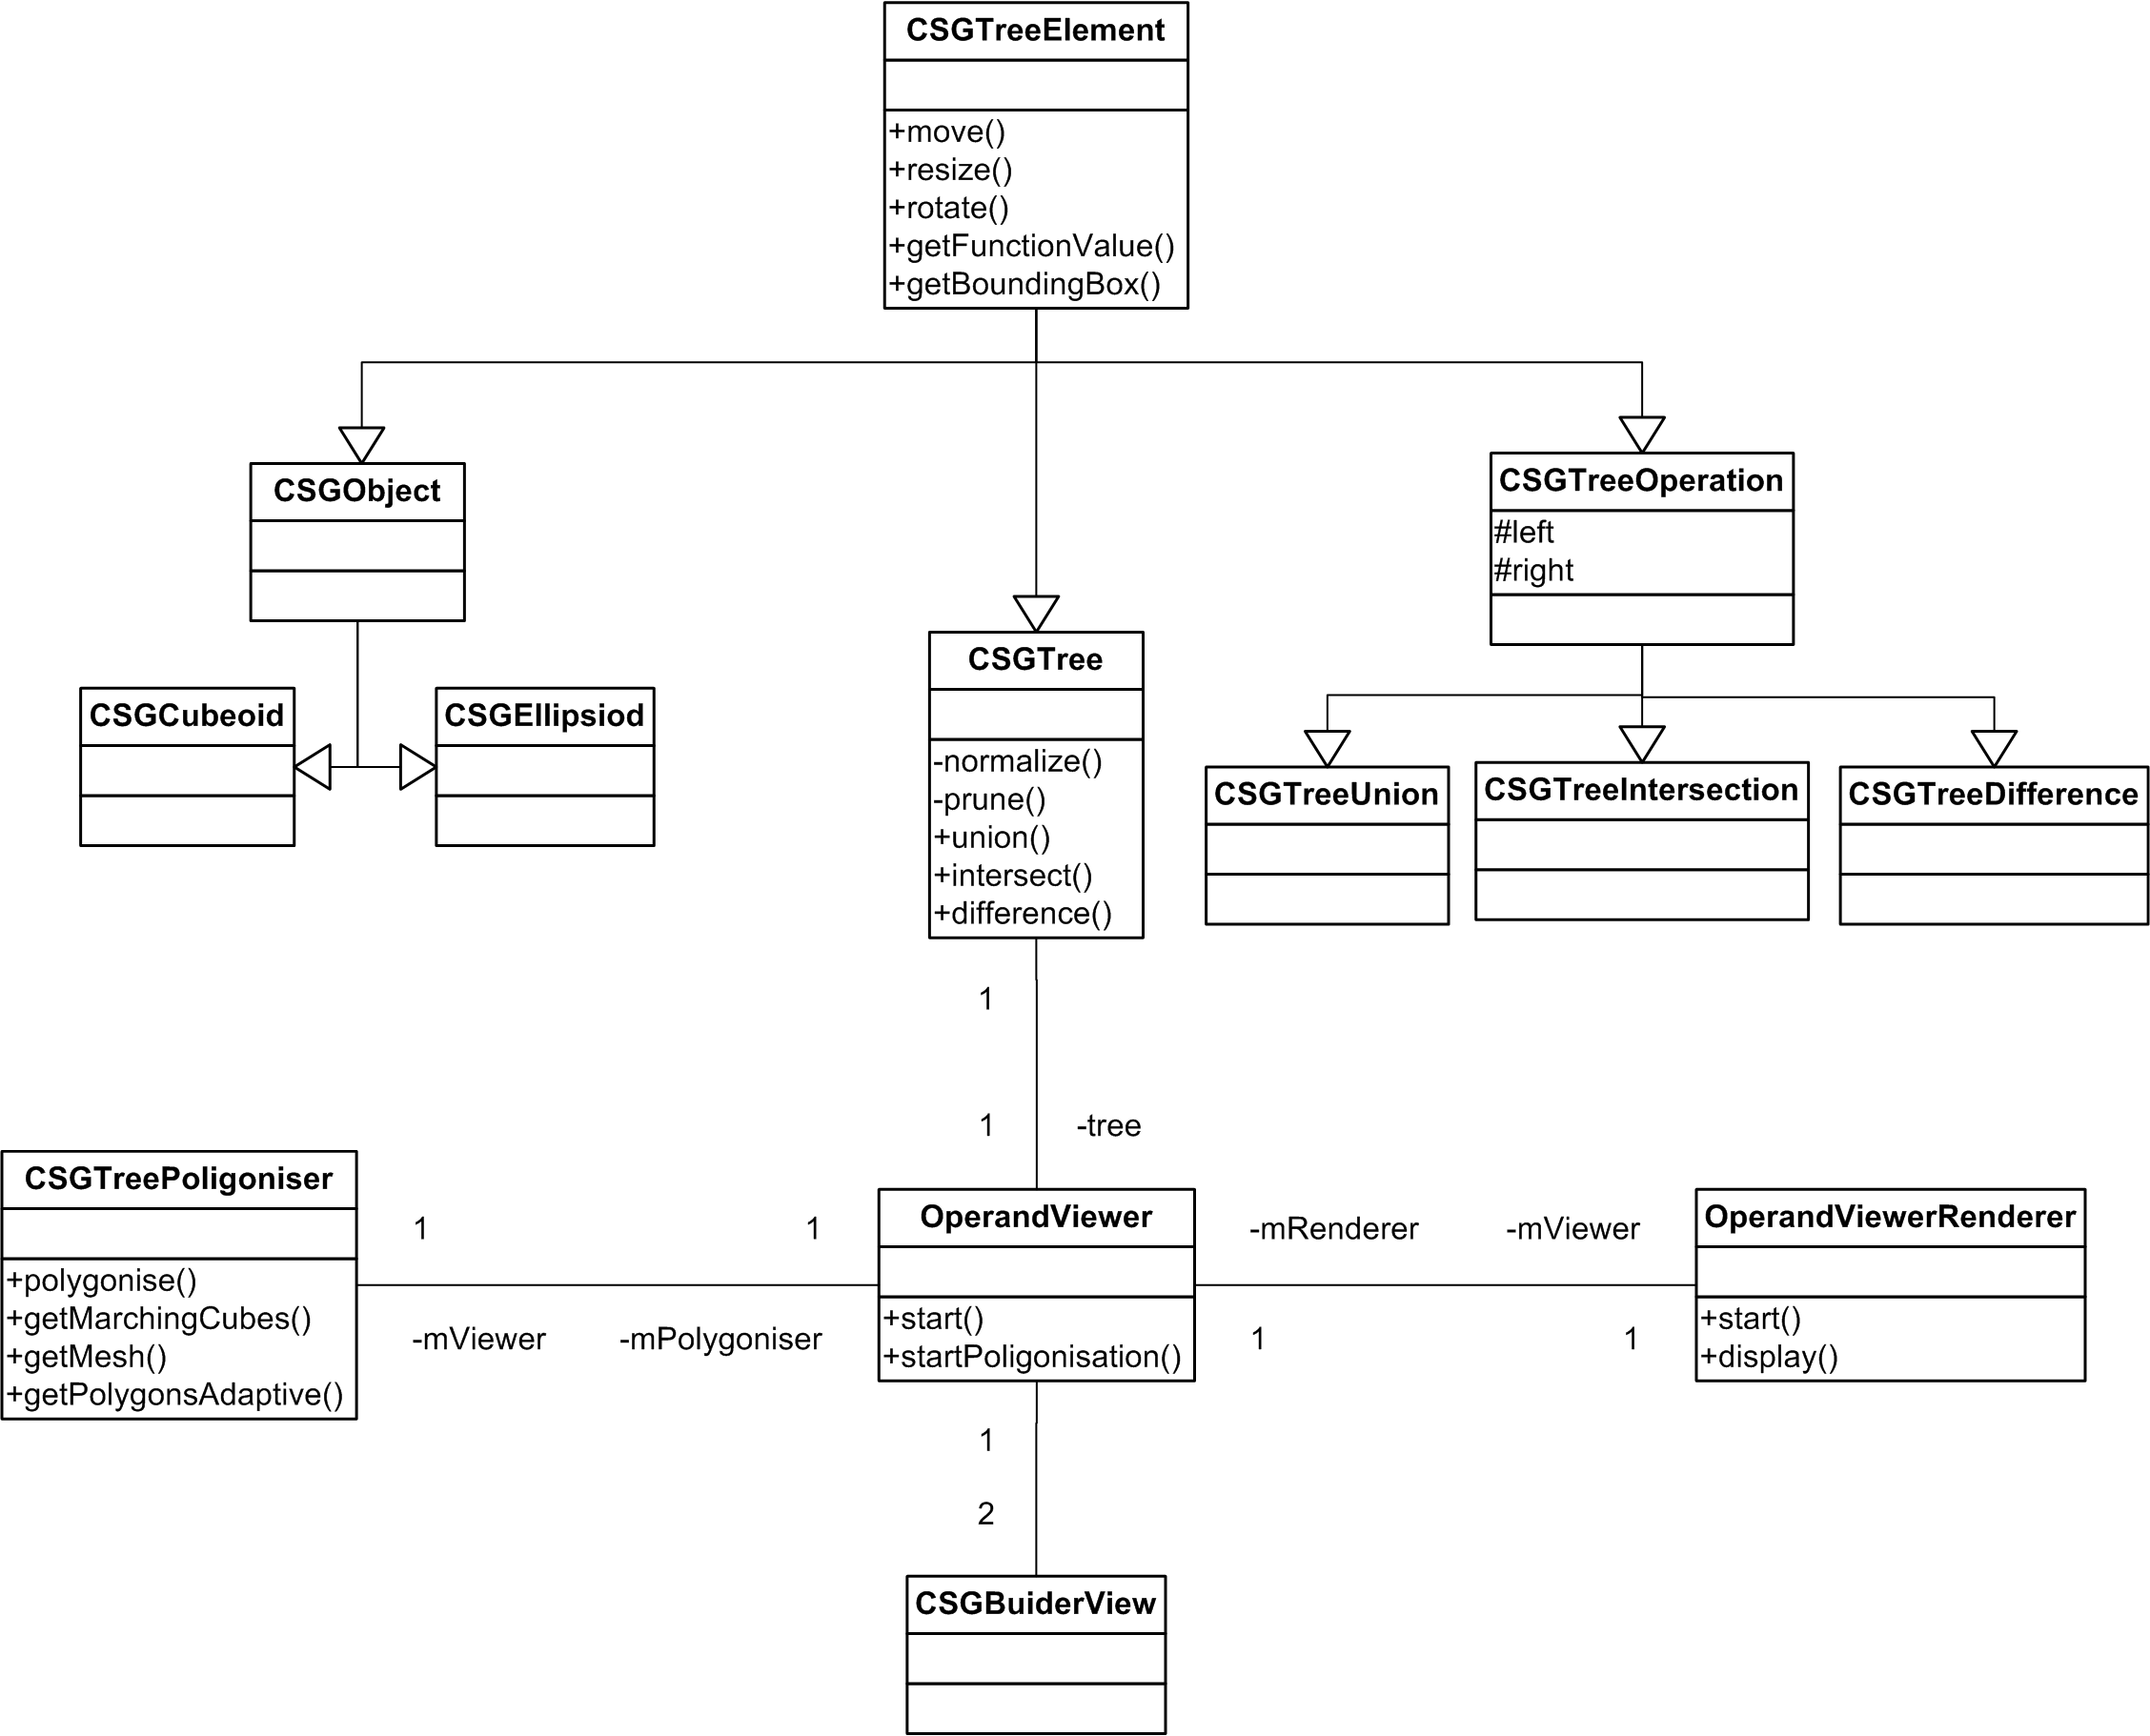
\includegraphics[width=\textwidth]{./images/architecture}
    \caption{The architecture of CSGBuilder}
    \label{figure:architecture}
\end{figure*}

The most important parts of the architecture of \emph{CSGBuilder} are shown in Figure~\ref{figure:architecture}. The figure is a simplified view of the architecture, but the most important classes and the most important fields and methods of these classes are included.

The classes in the figure can roughly be divided into two groups. A group which contains and manages the internal tree structure of objects, and a group which handles the rendering of objects.

The first group consists of the \texttt{CSGObject} class and its subclasses. The second group consists of \texttt{OperandViewer} class, the \texttt{CSGTreePolygoniser} class, the \texttt{OperandViewerRenderer}. The \texttt{CSGBuilderView} class is not part of these groups, because it implements the user interface of \emph{CSGBuilder}. The classes are described in more detail below.

\begin{list}{\labelitemi}{\leftmargin=0em}
    \item[] \textbf{CSGObject} This class defines an interface for all the nodes of a CSG tree. So, common operations that can be done on these nodes are defined here. The most important operations on a \texttt{CSGObject} are rotating the object around a point, resizing the object, moving the object to another position, calculate the value of an object given $x, y$ and $z$ coordinates and computing the bounding box of an object.
    \item[] \textbf{CSGTree} This class is an important descendant of \texttt{CSGObject}. This class implements operations on CSG trees such as the union, the intersection and the difference of a CSG tree and a CSGObject. Also, the normalization and pruning of the CSG tree is implemented in this class.
    \item[] \textbf{CSGTreeOperation} This class is the parent class of the \texttt{CSGTReeUnion}, \texttt{CSGTreeIntersection} and \texttt{CSGTreeDifference}. The most important part of this class are that a binary tree structure with a left and a right child are defined in this class. The behavior of the union, intersection and difference are defined in their corresponding classes.
    \item[] \textbf{CSGObject} This class defines basic properties for primitives. Its descendants \texttt{CSGCuboid} and \texttt{CSGEllipsoid} define specific behavior for the primitives in a CSG tree.
    \item[] \textbf{CSGTreePolygonizer} This class offers functionality to generate a mesh from a CSG tree.
    \item[] \textbf{OperandViewer} This class implements the panel on which a CSG tree is drawn. Here, some basic input functionality such as what happens at a mouse click is defined.
    \item[] \textbf{OperandViewerRenderer} This class implements all the rendering functions using OpenGL.
    \item[] \textbf{CSGBuilderView} As described before, this class implements the main functionality of the user interface of \emph{CSGBuilder}.
\end{list}

\section{Evaluation}
\label{sect:evaluation}

Due to time constraints we ended up dropping the following functionality:

\begin{itemize}
    \item[] \textbf{Performance} Originally we had planned to spend some time improving the performance, especially the marching cubes and the CSG tree algorithms. This means the final application is not as fast as we had imagined.
    \item[] \textbf{Crack problem} As described in section \ref{sect:crack_problem} our adaptive variant of the marching cubes algorithm suffers from the crack problem. We found a paper \cite{DMC} describing a technique to solve this using a dual grid, but we only got this partly working.
    \item[] \textbf{Object position/orientation} Currently changing the position and orientation at which the building block is removed from or added to the constructed object is only possible by changing the parameters for the building block object. Originally we had in mind that this could be done by zooming/rotating the object using the mouse.
    \item[] \textbf{Texturing} Texturing of the objects is not implemented.
\end{itemize}


\section{Conclusion}
\label{sect:conclusion}

\bibliographystyle{amsplain}
\begin{thebibliography}{99}
\bibitem{Wiegand96}
    T.~F.~Wiegand.\\
    Interactive Rendering of CSG Models.\\
    The Eurographics Association, 1996.

\bibitem{DMC}
    S. Schaefer, J. Warren. \\
    Dual Marching Cubes: Primal Contouring of Dual Grids. \\

\bibitem{img:wiki_csg_tree}
    Unknown author.\\
    Csg tree.png.\\
    http://en.wikipedia.org/wiki/File:Csg\_tree.png.\\
\end{thebibliography}
\end{document}
